

\begin{table}[ht]
\centering
\begin{tabular}{c|c|c|c|c}
Input Image & Histogram & Otsu Thresholding & Isodata Thresholding & Triangle Thresholding \\\hline
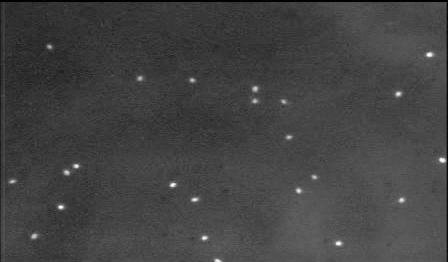
\includegraphics[scale=0.5]{Algae.png} & 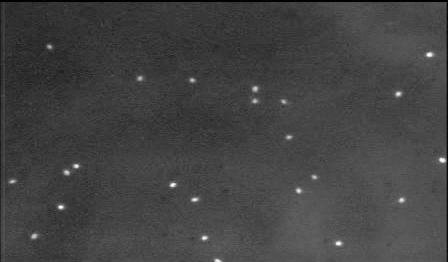
\includegraphics[scale=0.5]{Algae.png} & 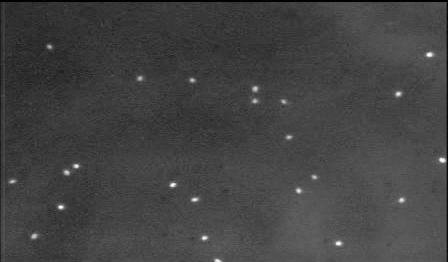
\includegraphics[scale=0.5]{Algae.png} & 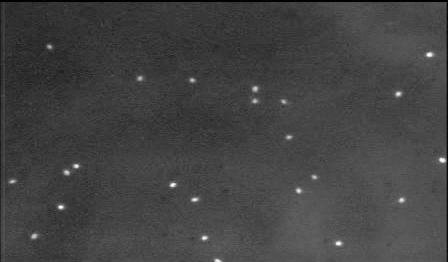
\includegraphics[scale=0.5]{Algae.png} & 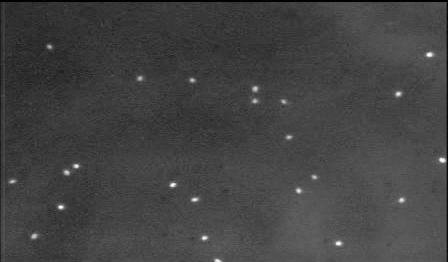
\includegraphics[scale=0.5]{Algae.png} \\
\end{tabular}
\caption{\label{tab:widgets}An example table.}
\end{table}

% TODO: difference between intermediate and final output images?

% The report can be
% written in Word, LaTeX, or a similar text processor, but must be submitted as a PDF and
% include your name and zID on the first page. It must also show the sample input images
% and the intermediate and final output images obtained. No templates are provided, but
% the report must be no more than 5 pages (A4), and must be single column, use 11 points
% Times New Roman or similar font, and have 2.5 cm margins.

% In your report, discuss the differences in the results and provide explanations (based on the
% histograms or otherwise) why for some images one thresholding technique may work betterthan others, 
% while for other images it may be the other way around.
% Present some general guidelines for which thresholding techniques are best for which kinds of images.
